\documentclass[12pt,a4paper]{report}

% ── Packages ──
\usepackage[utf8]{inputenc}
\usepackage[T1]{fontenc}
\usepackage{lmodern}
\usepackage[margin=1in, headheight=14pt]{geometry}
\usepackage{graphicx}
\usepackage{xcolor}
\usepackage{listings}
\usepackage{booktabs}
\usepackage{tabularx}
\usepackage{longtable}
\usepackage{hyperref}
\usepackage{fancyhdr}
\usepackage{titlesec}
\usepackage{tcolorbox}
\usepackage{enumitem}
\usepackage{amsmath}
\usepackage{float}
\usepackage{caption}
\usepackage{tikz}
\usetikzlibrary{shapes.geometric, arrows.meta, positioning, calc, fit}

% ── Colors ──
\definecolor{primaryblue}{HTML}{2563EB}
\definecolor{darkbg}{HTML}{1E293B}
\definecolor{codebg}{HTML}{F1F5F9}
\definecolor{accent}{HTML}{10B981}
\definecolor{warncolor}{HTML}{F59E0B}
\definecolor{codegreen}{HTML}{16A34A}
\definecolor{codegray}{HTML}{64748B}
\definecolor{codepurple}{HTML}{7C3AED}

% ── Hyperlinks ──
\hypersetup{
    colorlinks=true,
    linkcolor=primaryblue,
    urlcolor=primaryblue,
    citecolor=primaryblue
}

% ── Code Listings ──
\lstset{
    backgroundcolor=\color{codebg},
    basicstyle=\ttfamily\small,
    keywordstyle=\color{primaryblue}\bfseries,
    stringstyle=\color{codegreen},
    commentstyle=\color{codegray}\itshape,
    numberstyle=\tiny\color{codegray},
    numbers=left,
    numbersep=8pt,
    breaklines=true,
    frame=single,
    rulecolor=\color{codegray!30},
    tabsize=2,
    showstringspaces=false,
    captionpos=b
}

% ── Info Boxes ──
\newtcolorbox{conceptbox}[1][]{
    colback=primaryblue!5, colframe=primaryblue!70,
    fonttitle=\bfseries, title=#1, rounded corners
}
\newtcolorbox{warnbox}[1][]{
    colback=warncolor!8, colframe=warncolor!70,
    fonttitle=\bfseries, title=#1, rounded corners
}
\newtcolorbox{tipbox}[1][]{
    colback=accent!8, colframe=accent!70,
    fonttitle=\bfseries, title=#1, rounded corners
}

% ── Headers ──
\pagestyle{fancy}
\fancyhf{}
\fancyhead[L]{\small\textcolor{codegray}{P2P Energy Trading System}}
\fancyhead[R]{\small\textcolor{codegray}{\leftmark}}
\fancyfoot[C]{\thepage}
\renewcommand{\headrulewidth}{0.4pt}

% ── Title Formatting ──
\titleformat{\chapter}[display]
  {\normalfont\huge\bfseries\color{darkbg}}{Chapter \thechapter}{20pt}{\Huge}
\titleformat{\section}{\Large\bfseries\color{primaryblue}}{\thesection}{1em}{}
\titleformat{\subsection}{\large\bfseries\color{darkbg}}{\thesubsection}{1em}{}

% ══════════════════════════════════════════════════
\begin{document}

% ── Title Page ──
\begin{titlepage}
\centering
\vspace*{2cm}
{\Huge\bfseries\color{darkbg} Blockchain-Based\\[0.3cm]
Peer-to-Peer Energy\\[0.3cm]
Trading System\par}
\vspace{1cm}
{\LARGE\color{primaryblue} Complete Project Learning Guide\par}
\vspace{0.5cm}
{\large\color{codegray} With AI Load Prediction \& IoT Integration\par}
\vspace{2cm}

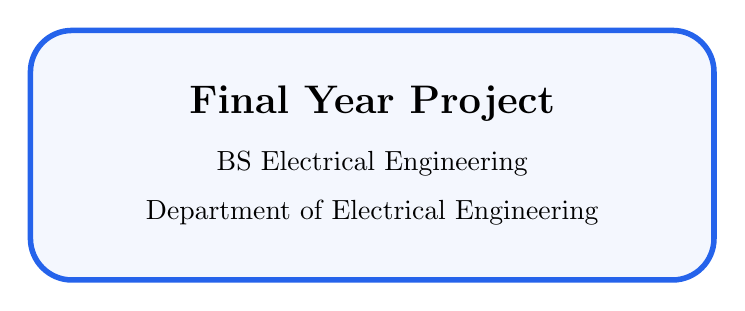
\begin{tikzpicture}
\node[draw=primaryblue, line width=2pt, rounded corners=15pt,
      inner sep=20pt, fill=primaryblue!5] {
    \begin{minipage}{0.6\textwidth}\centering
    \Large\bfseries
    Final Year Project\\[0.3cm]
    \normalsize\normalfont
    BS Electrical Engineering\\[0.2cm]
    Department of Electrical Engineering
    \end{minipage}
};
\end{tikzpicture}

\vfill
{\large\today\par}
\end{titlepage}

\tableofcontents
\newpage

% ══════════════════════════════════════════════════
% ══════════════════════════════════════════════════
\chapter{Project Ka Overview}
% ══════════════════════════════════════════════════

\section{Yeh Project Kya Hai?}

Yeh project \textbf{do gharon ke darmiyan bijli ka lein-dein (Peer-to-Peer Energy Trading)} karta hai. Is mein koi bechne wala company (jaise WAPDA/K-Electric) beech mein nahi hai --- seedha ghar se ghar bijli transfer hoti hai.

\begin{conceptbox}[Core Concept]
\textbf{House A} = Solar panel wala ghar (Producer) --- yeh bijli banata hai\\
\textbf{House B} = Consumer ghar --- yeh bijli leta hai\\[0.3cm]
Jab House A ki apni consumption kam ho ($\leq 1W$), toh \textbf{relay ON} ho jata hai aur extra bijli House B ko chali jati hai. Yeh sara record \textbf{blockchain} par permanently save hota hai, aur \textbf{AI model} agay ki consumption predict karta hai.
\end{conceptbox}

Iska matlab yeh hai ke agar House A mein koi appliance nahi chal raha (bijli ki zaroorat nahi), toh jo solar bijli ban rahi hai wo waste hone ke bajaye House B ko de di jati hai. Aur yeh sab kuch automatically hota hai --- kisi ko manually kuch karne ki zaroorat nahi.

\section{System Ke 5 Layers}

Poora system 5 alag-alag layers mein divide hai. Har layer ka apna kaam hai aur sab milke ek complete system banate hain:

\begin{table}[H]
\centering
\begin{tabularx}{\textwidth}{c l X}
\toprule
\textbf{\#} & \textbf{Layer} & \textbf{Kya Karta Hai} \\
\midrule
1 & Hardware (ESP32) & Bijli measure karta hai, relay control karta hai \\
2 & Backend (Node.js) & Sab data receive karta hai, APIs provide karta hai \\
3 & Blockchain (Solidity) & Transactions permanently record karta hai \\
4 & AI/ML (Python LSTM) & Agay ki consumption predict karta hai \\
5 & Dashboard (HTML/JS) & Browser mein sab kuch dikhata hai \\
\bottomrule
\end{tabularx}
\caption{System ke 5 Layers}
\end{table}

\textbf{Kyun 5 layers?} Kyunke har kaam alag hai. Sensor padhna alag kaam hai, data store karna alag, blockchain pe record karna alag, predict karna alag, aur dikhana alag. In sab ko ek mein mix karna galat approach hoti --- isliye modular design use ki hai.

\section{System Architecture}

\begin{figure}[H]
\centering
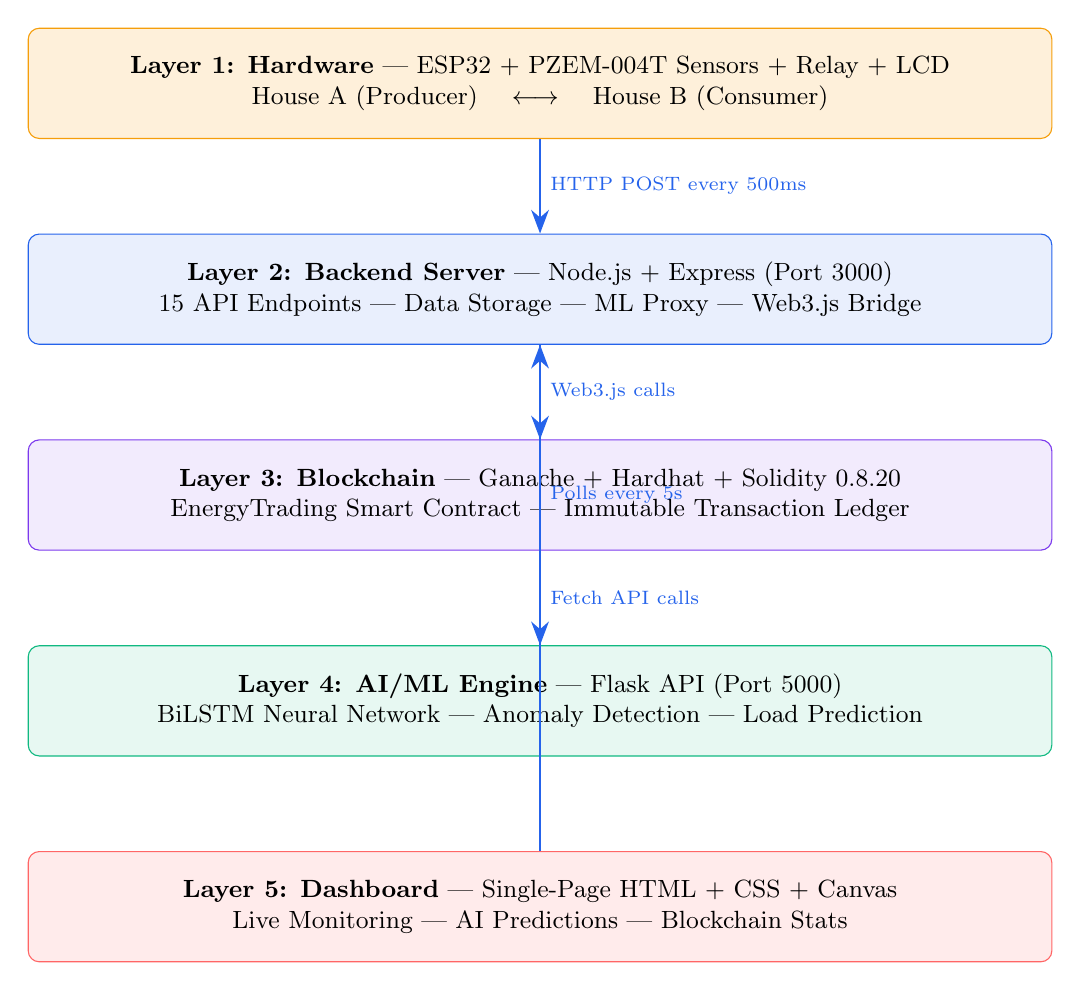
\begin{tikzpicture}[
    node distance=1.2cm,
    layer/.style={draw, rounded corners, minimum width=13cm, minimum height=1.4cm, align=center, font=\small},
    arrow/.style={-{Stealth[length=3mm]}, thick, primaryblue}
]
\node[layer, fill=warncolor!15, draw=warncolor] (hw) {\textbf{Layer 1: Hardware} --- ESP32 + PZEM-004T Sensors + Relay + LCD\\House A (Producer) \quad $\longleftrightarrow$ \quad House B (Consumer)};

\node[layer, fill=primaryblue!10, draw=primaryblue, below=of hw] (be) {\textbf{Layer 2: Backend Server} --- Node.js + Express (Port 3000)\\15 API Endpoints --- Data Storage --- ML Proxy --- Web3.js Bridge};

\node[layer, fill=codepurple!10, draw=codepurple, below=of be] (bc) {\textbf{Layer 3: Blockchain} --- Ganache + Hardhat + Solidity 0.8.20\\EnergyTrading Smart Contract --- Immutable Transaction Ledger};

\node[layer, fill=accent!10, draw=accent, below=of bc] (ml) {\textbf{Layer 4: AI/ML Engine} --- Flask API (Port 5000)\\BiLSTM Neural Network --- Anomaly Detection --- Load Prediction};

\node[layer, fill=red!8, draw=red!60, below=of ml] (ui) {\textbf{Layer 5: Dashboard} --- Single-Page HTML + CSS + Canvas\\Live Monitoring --- AI Predictions --- Blockchain Stats};

\draw[arrow] (hw) -- node[right, font=\scriptsize] {HTTP POST every 500ms} (be);
\draw[arrow] (be) -- node[right, font=\scriptsize] {Web3.js calls} (bc);
\draw[arrow] (be) -- node[right, font=\scriptsize] {Polls every 5s} (ml);
\draw[arrow] (ui) -- node[right, font=\scriptsize] {Fetch API calls} (be);

\end{tikzpicture}
\caption{5-Layer System Architecture}
\end{figure}

\textbf{Is diagram mein samjhne ki cheez yeh hai:} Sab kuch \textbf{backend server} se guzarta hai. ESP32 boards seedha blockchain se baat nahi karte --- wo apna data server ko bhejte hain, server usse blockchain pe record karta hai. Dashboard bhi seedha ESP32 se baat nahi karta --- wo bhi server se data leta hai. Server poore system ka \textbf{central hub} hai.

% ══════════════════════════════════════════════════
\chapter{Hardware Layer --- ESP32 Controllers}
% ══════════════════════════════════════════════════

\section{Hardware Ka Overall Picture}

System mein \textbf{2 ESP32 boards} hain --- ek House A ke liye (producer), ek House B ke liye (consumer). Dono ke saath \textbf{PZEM-004T} power sensor laga hua hai jo real-time mein voltage, current aur power measure karta hai.

\begin{tipbox}[Key Hardware Components]
\begin{itemize}[nosep]
    \item \textbf{ESP32 DevKit} --- WiFi-enabled microcontroller jo Arduino framework pe kaam karta hai
    \item \textbf{PZEM-004T v3.0} --- AC power monitor (voltage, current, power, energy, frequency, PF sab measure karta hai)
    \item \textbf{Relay Module} --- Active-LOW, 5V --- bijli ka raasta kholne/band karne ke liye
    \item \textbf{1602A LCD + I2C} --- Status display (sirf House A mein laga hai)
    \item \textbf{12V Charger + Inverter} --- Solar panel simulate karta hai (\textasciitilde10W AC output)
\end{itemize}
\end{tipbox}

% ──────────────────────────────────────────────────
\section{House A Controller --- Producer (Solar Wala Ghar)}

\subsection{Hardware Connections}

\begin{table}[H]
\centering
\begin{tabular}{l l l}
\toprule
\textbf{Component} & \textbf{ESP32 Pin} & \textbf{Note} \\
\midrule
PZEM TX wire & GPIO 18 & Sensor se data receive hota hai \\
PZEM RX wire & GPIO 19 & Sensor ko commands jate hain \\
Relay Control & GPIO 27 & Active-LOW (LOW=ON, HIGH=OFF) \\
LCD SDA & GPIO 21 & I2C data line \\
LCD SCL & GPIO 22 & I2C clock line (400kHz Fast Mode) \\
\bottomrule
\end{tabular}
\caption{House A Pin Connections}
\end{table}

\subsection{Solar Generation Model}

\begin{conceptbox}[Fixed Generation --- Kaise Kaam Karta Hai]
Solar panel real nahi hai --- 12V charger se simulate kiya gaya hai:
\begin{align*}
\text{DC Input} &= 12V \times 1A = 12W \\
\text{Inverter Efficiency} &= 80\% \text{ (HOPE H201)} \\
\text{AC Output} &= 12W \times 0.80 = \mathbf{10W} \text{ at 220V} \\
\text{Current} &= \frac{10W}{220V} \approx \mathbf{0.045A}
\end{align*}
\end{conceptbox}

\textbf{Kyun fixed hai?} Kyunke is prototype mein actual solar panel nahi laga --- 12V charger use hua hai jo hamesha 12W output deta hai. Inverter ki efficiency 80\% hai, toh AC side pe \textasciitilde10W aata hai. Yeh value code mein constant rakhi gayi hai, sensor se nahi padhti.

\subsection{Relay Decision Logic --- Sabse Important Cheez}

Yeh poore project ka \textbf{dil} hai. System yeh faisla karta hai:

\begin{enumerate}
    \item PZEM sensor se House A ki \textbf{actual consumption} padhta hai
    \item Agar consumption $\leq 1W$ hai (matlab koi appliance nahi chal raha) $\rightarrow$ \textbf{Relay ON} kar do
    \item Relay ON hone se bijli ka raasta khul jata hai aur 10W solar power House B ko flow hoti hai
    \item Agar consumption $> 1W$ ho jaye (koi appliance chala diya) $\rightarrow$ \textbf{Relay OFF} kar do
    \item Relay OFF hone se bijli ka raasta band --- House A apni solar power khud use kare ga
\end{enumerate}

\begin{warnbox}[Active-LOW Relay Ko Samjho]
Is relay mein logic \textbf{ulta} hai --- yeh beginners ke liye confusing hota hai:
\begin{itemize}[nosep]
    \item Pin ko \textbf{LOW} karo $\rightarrow$ Relay \textbf{ON} ho jata hai (bijli flow hoti hai)
    \item Pin ko \textbf{HIGH} karo $\rightarrow$ Relay \textbf{OFF} ho jata hai (bijli band)
\end{itemize}
Yeh isliye hai kyunke relay module ka internal circuit aise design hua hai. ``Active-LOW'' ka yehi matlab hai --- LOW signal pe activate hota hai.
\end{warnbox}

\subsection{Kya Kya Bhejta Hai Server Ko?}

House A ESP32 server ko \textbf{3 tarah ka data} bhejta hai, alag-alag waqfon pe:

\begin{table}[H]
\centering
\begin{tabularx}{\textwidth}{l l X}
\toprule
\textbf{Kab} & \textbf{Kahan} & \textbf{Kya Bhejta Hai} \\
\midrule
Har 500ms & \texttt{/api/live} & Voltage, current, power, relay status (live dashboard ke liye) \\
Har 60 seconds & \texttt{/api/transaction} & Energy transaction (sirf jab relay ON ho --- blockchain pe record hota hai) \\
Har 500ms & PZEM sensor read & Local variables mein store karta hai (server ko nahi bhejta, LCD pe dikhata hai) \\
\bottomrule
\end{tabularx}
\caption{House A Data Sending Schedule}
\end{table}

\textbf{Kyun 500ms?} Kyunke dashboard pe real-time feel chahiye. Agar 5 second pe bhejein toh lagta hai ke system slow hai. 500ms se dashboard bilkul live lagta hai.

\textbf{Kyun 60 seconds pe transaction?} Kyunke blockchain pe likhna \textbf{mehnga} hai (gas fee lagti hai). Agar har 500ms pe likhein toh bahut zyada gas kharcha ho. 60 seconds ek reasonable balance hai.

\subsection{LCD Display}

House A mein ek 16x2 LCD hai jo \textbf{3 screens rotate} karta hai har 3 seconds baad:

\begin{table}[H]
\centering
\begin{tabularx}{\textwidth}{c X}
\toprule
\textbf{Screen} & \textbf{Kya Dikhata Hai} \\
\midrule
1 & Consumption (Watts) + Relay ON/OFF + Excess power available \\
2 & Voltage + Current + Frequency + Power Factor \\
3 & Generation (10W) + Transaction count + Server/Blockchain/WiFi status \\
\bottomrule
\end{tabularx}
\caption{LCD ke 3 Screens}
\end{table}

\textbf{180° Rotation Support:} Agar LCD physically ulta (upside-down) lagaya hai mounting ke liye, toh ek setting ON karne se text automatically reverse ho jata hai aur rows swap ho jati hain. Yeh isliye banaya gaya ke prototype mein LCD ulta mount karna pada tha.

\textbf{Flicker-Free Design:} LCD mein ek common problem hai ``flicker'' --- jab screen clear karke dubara likhte hain toh jhilmilahaat aati hai. Is project mein \texttt{lcd.clear()} call nahi hoti --- poori 16-character row ek baar mein overwrite hoti hai, jis se koi flicker nahi aata.

\subsection{Smart Boot Detection}

\textbf{Problem tha:} Jab Arduino IDE ka Serial Monitor kholo toh ESP32 reset ho jata hai, aur poora startup sequence dubara chalta hai (WiFi connect, PZEM test, LCD messages). Yeh annoying hai.

\textbf{Solution:} ESP32 ke andar ek function hai jo bata sakta hai ke reset \textbf{kyun} hua --- power-on se ya software se. System detect karta hai ke agar yeh \textbf{pehli baar power mili hai} toh full startup chalao. Agar sirf Serial Monitor khula hai (software reset) toh seedha kaam pe lag jao.

\subsection{Ngrok Support}

\textbf{Problem:} ESP32 aur PC ek hi WiFi pe hone chahiyen. Agar alag hain toh communication nahi hogi.

\textbf{Solution:} Ngrok ek tool hai jo tumhare PC ka local server (\texttt{localhost:3000}) ko internet pe ek public HTTPS URL de deta hai. ESP32 us URL pe data bhejta hai, aur Ngrok usse tumhare PC tak pohancha deta hai. Firmware mein ek option hai --- agar Ngrok URL define karo toh HTTPS use kare ga, warna local IP pe HTTP use kare ga.

% ──────────────────────────────────────────────────
\section{House B Controller --- Consumer}

House B comparatively \textbf{simple} hai --- iska kaam sirf apni consumption monitor karna aur server ko bhejna hai.

\subsection{Hardware Connections}

\begin{table}[H]
\centering
\begin{tabular}{l l l}
\toprule
\textbf{Component} & \textbf{ESP32 Pin} & \textbf{Note} \\
\midrule
PZEM TX wire & GPIO 16 & Serial2 pe \\
PZEM RX wire & GPIO 17 & Serial2 pe \\
LED & GPIO 2 & Built-in LED (blink speed se status pata chalta hai) \\
\bottomrule
\end{tabular}
\caption{House B Pin Connections}
\end{table}

\subsection{Relay Detection --- Voltage Based}

\textbf{Problem:} House B ka ESP32 directly relay se connected nahi hai (relay House A mein hai). Toh House B ko kaise pata chalega ke relay ON hai ya OFF?

\textbf{Solution:} PZEM sensor ki \textbf{voltage reading} dekh kar. Jab relay ON hota hai toh House B ko voltage milti hai (\textgreater100V). Jab relay OFF hai toh voltage 0V aati hai. Yeh simple aur reliable method hai --- koi extra wire ya signal nahi chahiye.

\begin{table}[H]
\centering
\begin{tabular}{l l}
\toprule
\textbf{Voltage Reading} & \textbf{Matlab} \\
\midrule
$> 100V$ & Relay ON hai --- House A se bijli aa rahi hai \\
$< 10V$ & Relay OFF hai --- koi bijli nahi aa rahi \\
\bottomrule
\end{tabular}
\caption{Voltage-Based Relay Detection}
\end{table}

\subsection{LED Blink Pattern}

House B mein LCD nahi hai --- built-in LED ki blink speed se pata chalta hai kya ho raha hai:

\begin{itemize}[nosep]
    \item \textbf{Fast blink (har 250ms)} = House A se bijli mil rahi hai (relay ON)
    \item \textbf{Slow blink (har 1 second)} = Grid power pe hai (relay OFF)
\end{itemize}

\subsection{House B Kya Bhejta Hai?}

\begin{table}[H]
\centering
\begin{tabularx}{\textwidth}{l l X}
\toprule
\textbf{Kab} & \textbf{Kahan} & \textbf{Kya} \\
\midrule
Har 500ms & \texttt{/api/live} & Voltage, current, power, receiving status \\
Har 30 seconds & \texttt{/api/consumption} & Detailed consumption record (ML training ke liye) \\
\bottomrule
\end{tabularx}
\caption{House B Data Sending}
\end{table}

% ──────────────────────────────────────────────────
\section{Secrets Configuration --- Credentials}

Dono ESP32 boards ko WiFi password aur server address chahiye. Yeh sensitive information ek alag file (\texttt{secrets.h}) mein rakhi jati hai jo project ke saath share nahi hoti. Ek template file di gayi hai jis mein apne values fill karke use karna hota hai.

Is mein 3 cheezein set karni hoti hain:
\begin{enumerate}[nosep]
    \item \textbf{WiFi ka naam aur password} --- ESP32 internet se connect ho sake
    \item \textbf{Server ka IP address} --- ESP32 ko pata ho ke data kahan bhejna hai
    \item \textbf{Ngrok URL (optional)} --- Agar internet ke zariye communicate karna hai
\end{enumerate}

\begin{warnbox}[Security]
Yeh file kabhi Git mein commit nahi karni --- agar koi repository dekhe toh usse tumhara WiFi password nahi milna chahiye.
\end{warnbox}

% ══════════════════════════════════════════════════
\chapter{Backend Server --- Node.js}
% ══════════════════════════════════════════════════

\section{Server Ka Role --- Central Hub}

Backend server poore system ka \textbf{central hub} hai. Koi bhi component seedha kisi dusre se baat nahi karta --- sab server ke zariye hota hai.

\begin{conceptbox}[Server Kyun Zaroori Hai?]
\begin{itemize}[nosep]
    \item ESP32 boards apna data \textbf{server ko bhejte hain} (seedha blockchain ko nahi)
    \item Server wo data \textbf{blockchain pe record} karta hai (Web3.js ke zariye)
    \item Server har 5 second \textbf{AI server se prediction} mangta hai
    \item Dashboard browser mein khulta hai aur \textbf{server se data fetch} karta hai
    \item Server \textbf{CSV file maintain} karta hai jo AI training ke kaam aati hai
\end{itemize}
Matlab server ke bina kuch nahi chalta!
\end{conceptbox}

Server \textbf{Express.js} framework pe bana hai jo Node.js ka sabse popular web framework hai. Port \textbf{3000} pe chalta hai. 4 libraries use hoti hain: Express (web server), CORS (cross-origin requests), dotenv (config file), aur Web3.js (blockchain communication).

\section{API Endpoints --- Server Se Baat Kaise Hoti Hai}

Server ke \textbf{15 endpoints} hain. Endpoint matlab ek URL jis pe data bhej sakte ho ya mang sakte ho. In ko 3 categories mein samjho:

\subsection{Core Data Endpoints (Sensor Data Ke Liye)}

\begin{table}[H]
\centering
\begin{tabularx}{\textwidth}{l l X}
\toprule
\textbf{Method} & \textbf{URL} & \textbf{Kya Karta Hai Aur Kyun} \\
\midrule
POST & \texttt{/api/live} & ESP32 har 500ms pe yahan data bhejta hai. Server isse memory mein store karta hai (dashboard ke liye) aur CSV file mein bhi likhta hai (AI training ke liye). \\
GET & \texttt{/api/live} & Dashboard yahan se latest live readings leta hai --- voltage, current, power, relay status. \\
POST & \texttt{/api/transaction} & Jab relay ON ho toh House A har 60s pe yahan energy transaction bhejta hai. Server isse blockchain pe record karta hai. \\
POST & \texttt{/api/consumption} & House B har 30s pe apna consumption data yahan bhejta hai. Yeh AI training ke liye store hota hai. \\
GET & \texttt{/api/transactions} & Dashboard yahan se saari past transactions ki list leta hai. \\
GET & \texttt{/api/stats} & Total energy traded, average power, total value --- aggregated statistics. \\
\bottomrule
\end{tabularx}
\caption{Core Data Endpoints}
\end{table}

\textbf{POST vs GET samjho:} POST matlab tum server ko data \textbf{de} rahe ho (ESP32 readings bhej raha hai). GET matlab tum server se data \textbf{mang} rahe ho (dashboard readings le raha hai).

\subsection{AI/ML Proxy Endpoints}

\begin{table}[H]
\centering
\begin{tabularx}{\textwidth}{l l X}
\toprule
\textbf{Method} & \textbf{URL} & \textbf{Kya Karta Hai Aur Kyun} \\
\midrule
GET & \texttt{/api/predict} & AI prediction deta hai. Server pehle apna cache check karta hai --- agar fresh prediction available hai toh wahi de deta hai, warna Flask server se mangta hai. \\
GET & \texttt{/api/predict/history} & Pichli predictions ki list --- chart banane ke liye. \\
GET & \texttt{/api/ml/status} & AI server connected hai ya nahi, model loaded hai ya nahi, accuracy kitni hai. \\
GET & \texttt{/api/anomalies} & Koi abnormal reading aayi hai ya nahi (voltage spike, negative power, etc.). \\
\bottomrule
\end{tabularx}
\caption{AI Proxy Endpoints}
\end{table}

\textbf{Proxy kyun?} Dashboard seedha Flask server (port 5000) se baat kar sakta tha, lekin \textbf{proxy pattern} use kiya gaya hai --- matlab Node.js server beech mein hai. Iska faida yeh hai ke agar AI server band bhi ho toh dashboard crash nahi karta, server cached prediction de deta hai.

\subsection{Blockchain \& Export Endpoints}

\begin{table}[H]
\centering
\begin{tabularx}{\textwidth}{l l X}
\toprule
\textbf{Method} & \textbf{URL} & \textbf{Kya Karta Hai} \\
\midrule
GET & \texttt{/api/blockchain/status} & Ganache connected hai? Contract ka address kya hai? Kitne transactions hain? \\
GET & \texttt{/api/export/csv} & sensor\_log.csv file download karo (ML training ke liye) \\
GET & \texttt{/api/export/ml} & Transactions JSON format mein (ML ke liye) \\
\bottomrule
\end{tabularx}
\caption{Blockchain \& Export Endpoints}
\end{table}

\section{Data Storage --- 4 Files}

Server 4 files maintain karta hai jo runtime mein automatically banti aur update hoti hain:

\begin{table}[H]
\centering
\begin{tabularx}{\textwidth}{l X}
\toprule
\textbf{File} & \textbf{Kyun Hai Yeh} \\
\midrule
\texttt{transactions.json} & Blockchain transactions ka \textbf{local backup}. Agar blockchain band ho toh data yahan safe rehta hai. \\
\texttt{consumption.json} & House B ki consumption history. Last 10,000 records rakhta hai. \\
\texttt{sensor\_log.csv} & Yeh \textbf{sabse important file} hai --- AI model isi se seekhta hai. Har 500ms pe ek row add hoti hai jis mein dono houses ki readings hain. \\
\texttt{predictions.json} & AI predictions ki history. Last 500 predictions cache rehti hain. \\
\bottomrule
\end{tabularx}
\caption{Runtime Data Files}
\end{table}

\section{Blockchain Connection}

Server start hote hi Ganache blockchain se connect hone ki koshish karta hai. Agar connect ho jaye toh Web3.js ke zariye smart contract load karta hai. Jab ESP32 se transaction aata hai toh server us contract ka function call karta hai jo transaction permanently blockchain pe likh deta hai.

\begin{tipbox}[Graceful Fallback --- Yeh Smart Design Hai]
Agar Ganache band hai toh server crash \textbf{nahi} hota --- data sirf local JSON file mein save ho jata hai. Jab blockchain wapas connect ho, naye transactions wahan record honge. System hamesha kaam karta rehta hai chahe blockchain ho ya na ho.
\end{tipbox}

\section{ML Prediction Polling}

Server har \textbf{5 seconds} baad Flask AI server (port 5000) se ek prediction mangta hai. Flask server sensor\_log.csv ki latest data pe LSTM model chala ke bata hai ke aglay 1 minute mein kitni power use hogi.

Server yeh prediction \textbf{cache} kar leta hai. Jab dashboard maange toh cached result de deta hai --- har baar Flask se fresh nahi mangta. Agar Flask server band hai toh silently retry karta hai, koi error nahi aata dashboard pe.

\section{CSV Logging --- AI Data Collection}

Yeh system ki \textbf{sabse clever cheez} hai: jab bhi koi ESP32 live data bhejta hai, server us data ko ek CSV row mein convert karke file mein likh deta hai. Yeh file AI model ki training data hai. Matlab:

\begin{itemize}[nosep]
    \item System jitna \textbf{zyada chale ga}, utna zyada data collect hoga
    \item Zyada data $=$ AI model \textbf{zyada accurate} hoga
    \item Koi manually data collect karne ki zaroorat nahi --- \textbf{automatically} ho raha hai
\end{itemize}

Har CSV row mein 16 columns hain: timestamp, hour, day of week, House A ki 6 readings, House B ki 4 readings, relay state, receiving status, aur solar generation.

\section{Configuration}

Server ko ek \texttt{.env} file chahiye jis mein yeh information ho:

\begin{itemize}[nosep]
    \item \textbf{Ganache URL} --- Blockchain kahan chal rahi hai (default: \texttt{http://127.0.0.1:7545})
    \item \textbf{Contract Address} --- Deploy karne ke baad milta hai (deploy script automatically set karta hai)
    \item \textbf{Private Key} --- Ganache account ka key (transactions sign karne ke liye)
    \item \textbf{House Addresses} --- House A aur B ke Ethereum addresses
\end{itemize}

% ══════════════════════════════════════════════════
\chapter{Blockchain Layer --- Smart Contract}
% ══════════════════════════════════════════════════

\section{Blockchain Kya Hai? --- Simple Tareeqay Se Samjho}

\begin{conceptbox}[Blockchain = Permanent Record Book]
Socho ek register hai jis mein entry karne ke baad \textbf{kabhi mita nahi sakte, edit nahi kar sakte}. Har nayi entry ek ``block'' mein likhti hai, aur blocks ek chain ki tarah jud jaate hain --- isliye ``Blockchain''.

Is project mein hum Blockchain isliye use karte hain ke energy trading ka record \textbf{tamper-proof} ho. Koi yeh nahi keh sakta ke ``maine itni bijli nahi li thi'' --- record permanent hai.
\end{conceptbox}

\section{Tools Kya Use Hue Hain?}

\begin{table}[H]
\centering
\begin{tabularx}{\textwidth}{l X}
\toprule
\textbf{Tool} & \textbf{Kya Hai Aur Kyun Use Kiya} \\
\midrule
\textbf{Ganache} & Yeh ek \textbf{fake Ethereum blockchain} hai jo tumhare PC pe chalta hai. Real Ethereum pe deploy karna mehnga hai (gas fees lagti hain), isliye development ke liye Ganache use karte hain. Port 7545 pe chalta hai. \\
\textbf{Hardhat} & Yeh Solidity code ko compile karta hai aur blockchain pe deploy karta hai. Matlab yeh toh bas ek tool hai --- developer ka helper. \\
\textbf{Solidity 0.8.20} & Yeh wo programming language hai jis mein smart contract likha gaya hai. Solidity sirf Ethereum blockchain ke liye hai. \\
\textbf{Web3.js v4.3} & Yeh JavaScript library hai jo Node.js server ko blockchain se baat karne deti hai --- contract ke functions call karna, transactions bhejne ke liye. \\
\bottomrule
\end{tabularx}
\caption{Blockchain Tools Aur Unka Purpose}
\end{table}

\section{Smart Contract Kya Hai?}

Smart contract ek \textbf{program hai jo blockchain pe rehta hai}. Ek baar deploy karne ke baad isse koi change nahi kar sakta. Is project ka contract \textbf{EnergyTrading.sol} hai jo energy transactions record karta hai.

\begin{tipbox}[Real Life Analogy]
Smart contract ko aise samjho: ek vending machine. Tum paisa dalte ho, machine automatically samaan deti hai. Koi beech mein cheat nahi kar sakta. Smart contract bhi aise hi hai --- rules pehle se set hain, automatically execute hote hain.
\end{tipbox}

\section{Contract Mein Kya Data Store Hota Hai?}

Contract 2 tarah ka data rakhta hai:

\subsection{Transaction Record}

Har baar jab bijli transfer hoti hai, yeh information permanently save hoti hai:

\begin{table}[H]
\centering
\begin{tabularx}{\textwidth}{l X}
\toprule
\textbf{Field} & \textbf{Kya Hai} \\
\midrule
Transaction ID & Unique number (1, 2, 3, ...) \\
Seller Address & House A ka Ethereum address (0x1111...1111) \\
Buyer Address & House B ka Ethereum address (0x2222...2222) \\
Power (Watts) & Us waqt kitni watts transfer ho rahi thi \\
Energy (Wh) & Total kitni energy transfer hui (Watt-hours) \\
Price per kWh & Rate: 0.0001 ETH per kWh (roughly \$0.10) \\
Total Cost & Total paisa (Wei mein --- Ethereum ki sabse chhoti unit) \\
Timestamp & Kab hui yeh transaction \\
Solar Production & House A ki solar reading \\
House A Consumption & House A kitna use kar raha tha \\
\bottomrule
\end{tabularx}
\caption{Transaction Record Fields}
\end{table}

\subsection{House Information}

Har registered house ki information:

\begin{table}[H]
\centering
\begin{tabularx}{\textwidth}{l X}
\toprule
\textbf{Field} & \textbf{Kya Hai} \\
\midrule
Name & ``House\_A'' ya ``House\_B'' \\
Wallet Address & Ethereum address \\
Is Seller? & Haan (producer) ya Nahi (consumer) \\
Total Energy Traded & Ab tak kitni total energy trade ki \\
Transaction Count & Kitni transactions ki hain \\
\bottomrule
\end{tabularx}
\caption{House Information Fields}
\end{table}

\section{Contract Ke Main Functions}

\begin{table}[H]
\centering
\begin{tabularx}{\textwidth}{l X}
\toprule
\textbf{Function} & \textbf{Kya Karta Hai Aur Kyun} \\
\midrule
\texttt{recordTransaction()} & Naya energy trade record karta hai. Server yeh call karta hai jab ESP32 se transaction aata hai. Yeh permanently blockchain pe likh deta hai. \\
\texttt{getTransaction(id)} & Kisi purani transaction ko ID se dhundho. Dashboard isse dikhata hai. \\
\texttt{getLatestTransaction()} & Sabse haal ki transaction dekho. \\
\texttt{getTransactionCount()} & Total kitni transactions hain --- dashboard pe count dikhane ke liye. \\
\texttt{getStatistics()} & Total energy, total value, average power --- ek hi call mein sab stats mil jayen. \\
\texttt{getHouseInfo(address)} & Kisi house ki info dekho --- naam, role, total energy, TX count. \\
\texttt{setPricePerKwh()} & Bijli ki rate change karo. Sirf contract ka owner kar sakta hai. \\
\bottomrule
\end{tabularx}
\caption{Smart Contract Functions}
\end{table}

\section{Pricing --- Bijli Ka Rate Kaise Calculate Hota Hai?}

\begin{align*}
\text{Price per kWh} &= 0.0001 \text{ ETH} \approx \$0.10 \\
\text{Total Cost} &= \frac{\text{energyWh} \times \text{pricePerKwh}}{1000}
\end{align*}

\begin{tipbox}[Example]
Agar 10Wh energy transfer hui toh:\\
$\text{Cost} = \frac{10 \times 0.0001}{1000} = 0.000001 \text{ ETH}$\\[0.2cm]
Ganache pe yeh free hai (fake ETH hai), lekin real Ethereum pe yeh actual paisa hota.
\end{tipbox}

\section{Events --- Blockchain Notifications}

Contract 3 events emit karta hai. Event matlab ek notification jo blockchain pe permanently log hoti hai:

\begin{enumerate}[nosep]
    \item \textbf{HouseRegistered} --- Jab naya ghar register ho (constructor mein automatically hota hai)
    \item \textbf{EnergyTransferred} --- Jab bijli transfer ho (transaction ID, seller, buyer, power, energy, time)
    \item \textbf{TransactionRecorded} --- Block hash aur block number ke saath (verification ke liye)
\end{enumerate}

\textbf{Events kyun important hain?} Kyunke agar koi external application (jaise mobile app) blockchain monitor karna chahe toh events listen kar sakta hai --- real-time notifications milte hain.

\section{Deployment --- Contract Kaise Deploy Hota Hai?}

Ek deployment script hai jo 5 kaam karta hai:

\begin{enumerate}
    \item Solidity code ko \textbf{compile} karta hai (bytecode banata hai)
    \item Ganache pe \textbf{deploy} karta hai (bytecode blockchain pe upload hota hai)
    \item Contract address \textbf{save} karta hai ek JSON file mein
    \item Contract ka ABI (interface definition) \textbf{backend folder mein copy} karta hai --- taake server contract se baat kar sake
    \item Backend ki \texttt{.env} file mein contract address \textbf{automatically update} karta hai
\end{enumerate}

\begin{warnbox}[Ganache Reset = Re-deploy]
Har baar Ganache restart karne pe purani chain \textbf{mit jati hai}. Toh contract dubara deploy karna padta hai. Yeh sirf development mein hota hai --- real blockchain mein contract permanent hota hai.
\end{warnbox}

% ══════════════════════════════════════════════════
\chapter{AI / ML Layer --- Load Prediction}
% ══════════════════════════════════════════════════

\section{AI Ka Role Is Project Mein}

\begin{conceptbox}[AI Kya Karta Hai?]
AI model \textbf{predict} karta hai ke aglay 1 minute mein House A kitni bijli use kare ga. Agar predicted consumption $< 1W$ hai toh iska matlab hai relay ON rehna chahiye (bijli House B ko jaaye). Isse system \textbf{pehle se} faisla kar sakta hai --- react karne ki bajaye \textbf{proactively} kaam karta hai.
\end{conceptbox}

\section{LSTM Kya Hai? --- Simple Explanation}

\begin{conceptbox}[LSTM = Memory Wala Neural Network]
Normal neural network sirf ek waqt ki cheez dekhta hai. LSTM (Long Short-Term Memory) \textbf{time ki chain} dekhta hai --- yeh yaad rakhta hai ke ``pichlay 10 seconds mein kya hua'' aur us pattern se agay ka predict karta hai.\\[0.3cm]
\textbf{Example:} Agar pichlay 10 seconds mein power dheere dheere badh rahi hai (0.5W, 0.7W, 1.2W, 1.8W...), toh LSTM samajh jaye ga ke agay aur badhegi --- aur relay OFF karne ka predict kare ga.\\[0.3cm]
\textbf{Bidirectional} ka matlab hai ke model dono taraf se dekhta hai --- aagay se bhi, peechay se bhi --- jis se aur accurate hota hai.
\end{conceptbox}

\section{Data --- AI Kahan Se Seekhta Hai?}

AI model \texttt{sensor\_log.csv} file se seekhta hai. Yeh file do tareeqon se banti hai:

\begin{enumerate}
    \item \textbf{Real Data:} Jab hardware chal raha ho --- server har 500ms pe ek CSV row likhta hai (automatically)
    \item \textbf{Synthetic Data:} Ek Python script (\texttt{generate\_data.py}) fake lekin realistic data bana deti hai --- jab hardware available na ho tab training ke liye kaam aata hai
\end{enumerate}

\section{Training Pipeline --- 10 Steps Mein Model Kaise Banta Hai}

\begin{table}[H]
\centering
\begin{tabularx}{\textwidth}{c X}
\toprule
\textbf{Step} & \textbf{Kya Hota Hai Aur Kyun} \\
\midrule
1 & \textbf{CSV Load:} sensor\_log.csv file padhta hai --- yeh raw data hai \\
2 & \textbf{Outlier Removal:} Agar koi reading bahut unusual hai (sensor glitch) toh hatata hai. IQR method use hota hai --- agar koi value normal range se 3 guna zyada door hai toh remove. \\
3 & \textbf{Smoothing:} PZEM sensor mein thoda noise hota hai (readings jump karti hain). Rolling average lagata hai (5 readings ka average) taake data smooth ho. \\
4 & \textbf{Feature Selection:} 16 columns mein se sirf \textbf{11 kaam ki columns} choose karta hai (neeche table mein). \\
5 & \textbf{Normalize:} Sab values ko 0 se 1 ke beech laata hai. \textbf{Kyun?} Kyunke voltage 220 hai aur current 0.045 --- itna bara farq model ko confuse karta hai. Normalize karne se sab barabar scale pe aa jate hain. \\
6 & \textbf{Sequences:} 20 consecutive rows ka ek group banata hai (input) aur 1 minute baad ki power value target hoti hai (output). Yeh LSTM ko ``time ka pattern'' dikhata hai. \\
7 & \textbf{Split:} Data ko 3 hisson mein todta hai --- 70\% training, 15\% validation, 15\% testing. \\
8 & \textbf{Train:} BiLSTM model ko 80 epochs tak train karta hai (ek epoch = poora data ek baar dekh liya). \\
9 & \textbf{Evaluate:} Test data pe accuracy check karta hai --- MAE, RMSE, MAPE calculate karta hai. \\
10 & \textbf{Save:} Trained model, scaler, aur metadata files save karta hai. \\
\bottomrule
\end{tabularx}
\caption{Complete Training Pipeline}
\end{table}

\section{11 Features --- Model Ko Kya Input Milta Hai?}

\begin{table}[H]
\centering
\begin{tabularx}{\textwidth}{c l X}
\toprule
\textbf{\#} & \textbf{Feature} & \textbf{Kyun Important Hai} \\
\midrule
1 & House A Voltage & Voltage se load pattern pata chalta hai \\
2 & House A Current & Current consumption ka direct measure \\
3 & House A Power & \textbf{TARGET --- yeh predict karna hai!} \\
4 & House A Frequency & Grid stability indicator (50Hz normal) \\
5 & House A Power Factor & Kitni efficiently bijli use ho rahi hai \\
6 & House B Power & Dusre ghar ki demand se correlation ho sakta hai \\
7 & House B Current & House B current reading \\
8 & Relay State & Relay ON/OFF --- directly affects power flow \\
9 & Receiving from A & House B receive kar raha hai ya nahi \\
10 & Hour (0-23) & \textbf{Waqt bahut important hai} --- subah aur raat mein consumption alag hoti hai \\
11 & Day of Week & Weekday/weekend pe usage pattern alag hota hai \\
\bottomrule
\end{tabularx}
\caption{Model Input Features Aur Unki Importance}
\end{table}

\section{Model Architecture}

Model ka design:

\begin{figure}[H]
\centering
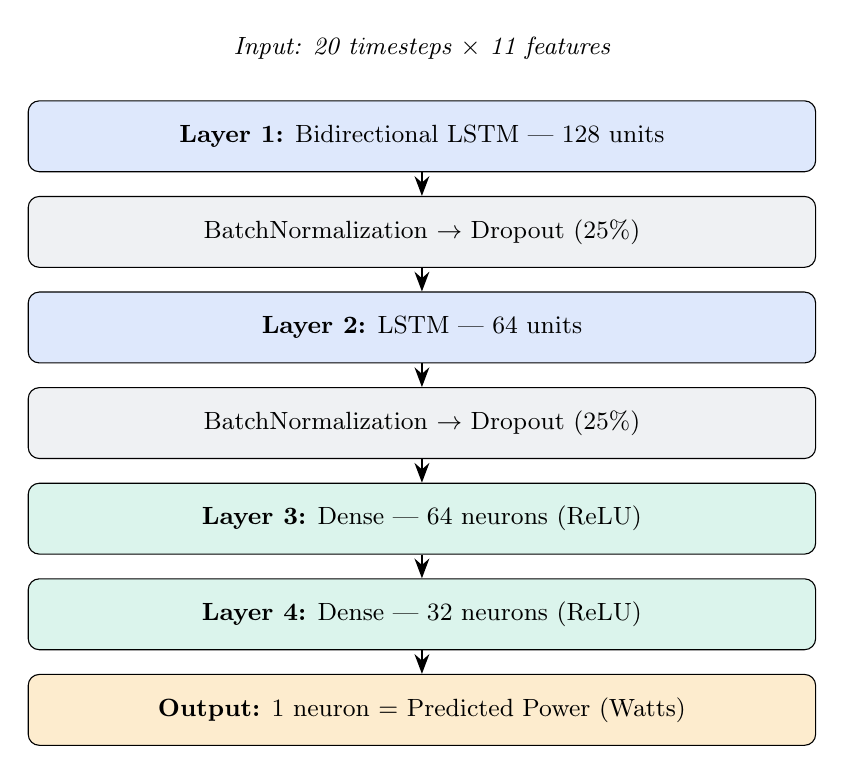
\begin{tikzpicture}[
    layer/.style={draw, rounded corners, minimum width=10cm, minimum height=0.9cm, align=center, font=\small},
    arrow/.style={-{Stealth[length=2.5mm]}, thick}
]
\node[layer, fill=primaryblue!15] (l1) {\textbf{Layer 1:} Bidirectional LSTM --- 128 units};
\node[layer, fill=codegray!10, below=0.3cm of l1] (bn1) {BatchNormalization $\rightarrow$ Dropout (25\%)};
\node[layer, fill=primaryblue!15, below=0.3cm of bn1] (l2) {\textbf{Layer 2:} LSTM --- 64 units};
\node[layer, fill=codegray!10, below=0.3cm of l2] (bn2) {BatchNormalization $\rightarrow$ Dropout (25\%)};
\node[layer, fill=accent!15, below=0.3cm of bn2] (d1) {\textbf{Layer 3:} Dense --- 64 neurons (ReLU)};
\node[layer, fill=accent!15, below=0.3cm of d1] (d2) {\textbf{Layer 4:} Dense --- 32 neurons (ReLU)};
\node[layer, fill=warncolor!20, below=0.3cm of d2] (out) {\textbf{Output:} 1 neuron = Predicted Power (Watts)};

\node[above=0.4cm of l1, font=\small\itshape] {Input: 20 timesteps $\times$ 11 features};

\draw[arrow] (l1) -- (bn1);
\draw[arrow] (bn1) -- (l2);
\draw[arrow] (l2) -- (bn2);
\draw[arrow] (bn2) -- (d1);
\draw[arrow] (d1) -- (d2);
\draw[arrow] (d2) -- (out);
\end{tikzpicture}
\caption{BiLSTM Model Architecture}
\end{figure}

\textbf{Har layer kya kar rahi hai:}

\begin{itemize}
    \item \textbf{Bidirectional LSTM (128 units):} Yeh main layer hai --- 20 timesteps ka pattern samajhti hai, aagay aur peechay dono directions se
    \item \textbf{BatchNormalization:} Data ko stable rakhti hai training ke dauraan --- isse model tezi se seekhta hai
    \item \textbf{Dropout (25\%):} Training mein randomly 25\% neurons band kar deti hai --- isse model \textbf{overfitting} se bachta hai (matlab sirf training data ratta nahi marta, generalize karta hai)
    \item \textbf{LSTM (64 units):} Doosri LSTM layer jo pehli layer ke output ko aur refine karti hai
    \item \textbf{Dense (64, 32):} Regular neural network layers jo final prediction ke liye combine karti hain
    \item \textbf{Output (1 neuron):} Ek single number --- predicted power in Watts
\end{itemize}

\section{Training Ke Smart Features}

\begin{table}[H]
\centering
\begin{tabularx}{\textwidth}{l X}
\toprule
\textbf{Feature} & \textbf{Kya Karta Hai Aur Kyun} \\
\midrule
Early Stopping & Agar 12 epochs mein model ki accuracy improve nahi ho rahi toh training \textbf{ruk jati hai}. Isse time waste nahi hota aur overfitting se bachta hai. \\
Model Checkpoint & Har epoch ke baad check karta hai --- agar yeh best result hai toh model save kar lo. Final mein \textbf{sabse best wala model} milta hai, chahe training ke end pe worse ho jaye. \\
Learning Rate Reduction & Agar 6 epochs mein improvement nahi toh learning rate \textbf{aadhi} kar do. Yeh model ko fine-tune karne mein madad karta hai --- jab bade steps se improvement nahi ho rahi toh chhote steps try karo. \\
\bottomrule
\end{tabularx}
\caption{Smart Training Features}
\end{table}

\section{Prediction Server --- Flask API}

Trained model ko use karne ke liye ek Flask server chalta hai port \textbf{5000} pe. Node.js backend har 5 seconds baad is se prediction mangta hai.

\subsection{Prediction Kaise Hota Hai?}

\begin{enumerate}
    \item Server \texttt{sensor\_log.csv} ki \textbf{last 100 rows} padhta hai
    \item Us mein se 11 feature columns select karta hai
    \item MinMaxScaler se values ko \textbf{0--1 ke beech normalize} karta hai (wahi scaler jo training mein use hua tha)
    \item Last \textbf{20 rows ka sequence} banata hai (model ko 20 timesteps chahiyen)
    \item LSTM model pe \texttt{predict()} chalaata hai --- ek normalized number aata hai
    \item Us number ko \textbf{inverse transform} karta hai --- wapas real Watts mein convert karta hai
    \item \textbf{Confidence} calculate karta hai --- agar recent data stable hai toh confidence zyada, agar bahut vary kar raha hai toh kam
    \item \textbf{Relay prediction:} Agar predicted power $< 1W$ toh relay ON rehna chahiye, warna OFF
\end{enumerate}

\subsection{Anomaly Detection}

Server har prediction ke saath readings mein \textbf{anomalies} (abnormal values) bhi check karta hai:

\begin{table}[H]
\centering
\begin{tabularx}{\textwidth}{l l l X}
\toprule
\textbf{Type} & \textbf{Condition} & \textbf{Severity} & \textbf{Kyun Problem Hai} \\
\midrule
Power spike & $> 9.5W$ & Warning & Generation sirf 10W hai --- 9.5W consumption matlab almost sab use ho raha hai \\
Negative power & $< -0.1W$ & Critical & Bijli negative nahi ho sakti --- sensor mein fault hai \\
Overvoltage & $> 250V$ & Critical & 220V normal hai --- 250+ se equipment damage ho sakti hai \\
Undervoltage & $< 180V$ & Warning & Bahut kam voltage --- appliances properly kaam nahi karenge \\
\bottomrule
\end{tabularx}
\caption{Anomaly Detection Rules}
\end{table}

\section{Accuracy Metrics --- Model Kitna Sahi Hai?}

\begin{table}[H]
\centering
\begin{tabularx}{\textwidth}{l l X}
\toprule
\textbf{Metric} & \textbf{Formula} & \textbf{Matlab Kya Hai} \\
\midrule
MAE & $\frac{1}{n}\sum|actual - predicted|$ & Average error Watts mein. Agar MAE = 0.5W hai toh model average 0.5W galat hai. \\
RMSE & $\sqrt{\frac{1}{n}\sum(actual - predicted)^2}$ & Bade errors ko zyada penalize karta hai. Agar kabhi kabhi bahut galat hai toh RMSE zyada hoga. \\
MAPE & $\frac{100}{n}\sum\left|\frac{actual - predicted}{actual}\right|$ & Percentage mein error. 5\% MAPE matlab average 5\% galat. \\
\bottomrule
\end{tabularx}
\caption{Model Accuracy Metrics}
\end{table}

\begin{tipbox}[Good Accuracy Values]
Is project ke liye: MAE $< 0.5W$ aur MAPE $< 10\%$ excellent hai. Kyunke total generation sirf 10W hai, toh 0.5W error acceptable hai.
\end{tipbox}

% ══════════════════════════════════════════════════
\chapter{Dashboard --- Web Interface}
% ══════════════════════════════════════════════════

\section{Dashboard Ka Overview}

Dashboard ek \textbf{single HTML page} hai jo browser mein khulta hai (\texttt{http://localhost:3000}). Yeh poore system ka visual interface hai --- sab kuch yahan dikhta hai.

\begin{conceptbox}[Dashboard Kyun Zaroori Hai?]
Bina dashboard ke tumhe terminal/console dekhna padta. Dashboard se ek nazar mein pata chal jata hai:
\begin{itemize}[nosep]
    \item Dono houses kitni bijli use kar rahe hain
    \item Relay ON hai ya OFF
    \item AI kya predict kar raha hai
    \item Blockchain pe kitni transactions hui hain
    \item Koi anomaly toh nahi aayi
\end{itemize}
\end{conceptbox}

\section{Design Choices --- Kyun Aise Banaya}

\begin{table}[H]
\centering
\begin{tabularx}{\textwidth}{l X}
\toprule
\textbf{Choice} & \textbf{Kyun} \\
\midrule
\textbf{Dark Theme} & Energy monitoring systems typically dark hote hain (jaise control rooms). Readings zyada clearly dikhti hain dark background pe. \\
\textbf{Single HTML File} & Setup simple rakhne ke liye. Koi build process nahi, koi framework nahi --- sirf ek file hai, server ke saath serve hoti hai. \\
\textbf{No External JS Libraries} & Chart.js ya React use karne se 200KB+ extra load hota. Hamara custom Canvas chart sirf 100 lines mein hai aur perfectly kaam karta hai. Zero dependencies = zero problems. \\
\textbf{Inter Font} & Professional aur modern dikhta hai. Google Fonts se load hota hai. \\
\textbf{Responsive Layout} & Mobile pe bhi properly dikhta hai (1-column layout), desktop pe multi-column. \\
\bottomrule
\end{tabularx}
\caption{Design Decisions}
\end{table}

\section{Dashboard Ke 8 Sections}

\begin{table}[H]
\centering
\begin{tabularx}{\textwidth}{c l X}
\toprule
\textbf{\#} & \textbf{Section} & \textbf{Kya Dikhata Hai Aur Kyun} \\
\midrule
1 & \textbf{Navbar} & 3 status badges: Blockchain (green/red), AI Engine (green/red), Live Feed (green/red). Ek nazar mein pata chal jata hai ke kya chal raha hai kya nahi. \\
2 & \textbf{Live Monitoring} & House A aur B ki readings --- Voltage, Current, Power, Relay status. Har 500ms pe update hota hai. \\
3 & \textbf{AI Prediction} & 3 cards: Predicted power (aglay 1 min), Relay prediction (ON/OFF hona chahiye), Model accuracy (confidence bar ke saath). \\
4 & \textbf{Chart} & Actual vs Predicted power ka line chart. Blue line = actual, purple dashed = predicted. Isse dikhta hai model kitna close hai. \\
5 & \textbf{ML Model Status} & Model ki technical info: MAE, RMSE, MAPE, version, training date, total predictions count. \\
6 & \textbf{Anomaly Alerts} & Agar koi abnormal reading aaye (voltage spike, negative power, etc.) toh yahan warning dikhti hai. \\
7 & \textbf{Blockchain Stats} & Contract address, total transactions, total energy traded, network info. \\
8 & \textbf{Transactions} & Recent transactions ki list --- har ek mein TX hash, power, energy, timestamp dikhta hai. \\
\bottomrule
\end{tabularx}
\caption{Dashboard Ke 8 Sections}
\end{table}

\section{Data Polling --- Dashboard Data Kaise Leta Hai?}

Dashboard continuously server se data \textbf{fetch} karta rehta hai. 2 alag speeds pe:

\begin{table}[H]
\centering
\small
\begin{tabularx}{\textwidth}{l l X}
\toprule
\textbf{Interval} & \textbf{Kya Fetch Hota Hai} & \textbf{Kyun Itni Speed} \\
\midrule
\textbf{Har 500ms} & Live sensor readings (House A, B) & Real-time feel chahiye --- 500ms se lagta hai ke values ``live'' hain \\
\textbf{Har 5s} & AI prediction, ML status, anomalies, blockchain, transactions & Yeh data slowly change hota hai, 5s kaafi hai \\
\bottomrule
\end{tabularx}
\caption{Dashboard Polling Intervals}
\end{table}

\textbf{Kyun 2 alag speeds?} Kyunke live readings har 500ms pe change hoti hain (sensor data), toh fast polling chahiye. Lekin blockchain stats ya AI prediction har second nahi badalta --- 5 seconds pe ek baar kaafi hai. Isse \textbf{network bandwidth bhi bach'ti hai} aur server pe load bhi kam hota hai.

\section{Custom Canvas Chart}

Dashboard mein ek chart hai jo \textbf{Actual power} (blue line) aur \textbf{Predicted power} (purple dashed line) ko overlay karke dikhata hai.

Yeh chart \textbf{pure Canvas 2D API} se bana hai --- koi library nahi. Iska faida:
\begin{itemize}[nosep]
    \item Zero extra file load (Chart.js = 200KB+, hamara = 0 extra)
    \item Exactly wahi design jo chahiye tha (dark theme matching)
    \item Last 50 data points dikhata hai (older automatically hat jaate hain)
\end{itemize}

Har 5 seconds pe jab nayi prediction aati hai, chart mein ek nayi point add hoti hai --- actual aur predicted dono ki.

% ══════════════════════════════════════════════════
\chapter{Complete Data Flow}
% ══════════════════════════════════════════════════

\section{End-to-End --- Poora System Kaise Chalta Hai}

Ab sab layers samajh aaye hain, toh dekhte hain ke \textbf{sab milke kaise kaam karte hain} --- shuru se aakhir tak:

\begin{figure}[H]
\centering
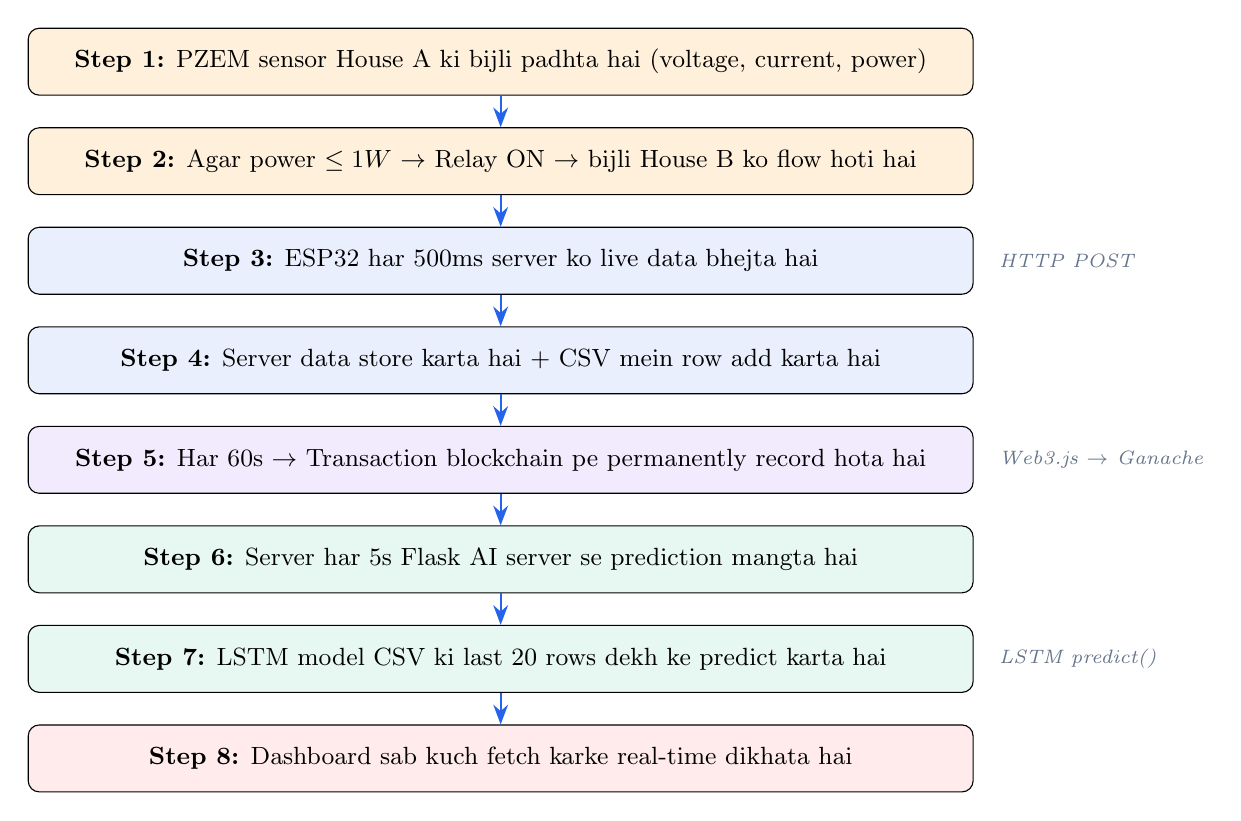
\begin{tikzpicture}[
    flowstep/.style={draw, rounded corners, minimum width=12cm, minimum height=0.85cm, align=center, font=\small},
    arrow/.style={-{Stealth[length=2.5mm]}, thick, primaryblue},
    note/.style={font=\scriptsize\itshape, text=codegray}
]

\node[flowstep, fill=warncolor!15] (s1) {\textbf{Step 1:} PZEM sensor House A ki bijli padhta hai (voltage, current, power)};
\node[flowstep, fill=warncolor!15, below=0.4cm of s1] (s2) {\textbf{Step 2:} Agar power $\leq 1W$ $\rightarrow$ Relay ON $\rightarrow$ bijli House B ko flow hoti hai};
\node[flowstep, fill=primaryblue!10, below=0.4cm of s2] (s3) {\textbf{Step 3:} ESP32 har 500ms server ko live data bhejta hai};
\node[flowstep, fill=primaryblue!10, below=0.4cm of s3] (s4) {\textbf{Step 4:} Server data store karta hai + CSV mein row add karta hai};
\node[flowstep, fill=codepurple!10, below=0.4cm of s4] (s5) {\textbf{Step 5:} Har 60s $\rightarrow$ Transaction blockchain pe permanently record hota hai};
\node[flowstep, fill=accent!10, below=0.4cm of s5] (s6) {\textbf{Step 6:} Server har 5s Flask AI server se prediction mangta hai};
\node[flowstep, fill=accent!10, below=0.4cm of s6] (s7) {\textbf{Step 7:} LSTM model CSV ki last 20 rows dekh ke predict karta hai};
\node[flowstep, fill=red!8, below=0.4cm of s7] (s8) {\textbf{Step 8:} Dashboard sab kuch fetch karke real-time dikhata hai};

\draw[arrow] (s1) -- (s2);
\draw[arrow] (s2) -- (s3);
\draw[arrow] (s3) -- (s4);
\draw[arrow] (s4) -- (s5);
\draw[arrow] (s5) -- (s6);
\draw[arrow] (s6) -- (s7);
\draw[arrow] (s7) -- (s8);

\node[note, right=0.2cm of s3] {HTTP POST};
\node[note, right=0.2cm of s5] {Web3.js $\rightarrow$ Ganache};
\node[note, right=0.2cm of s7] {LSTM predict()};

\end{tikzpicture}
\caption{Complete Data Flow --- Step by Step}
\end{figure}

\section{House B Ka Parallel Flow}

House B \textbf{simultaneously} (saath saath) apna data bhejta hai:

\begin{enumerate}[nosep]
    \item PZEM sensor se voltage padhta hai --- agar $> 100V$ toh samajh jata hai ke relay ON hai
    \item Har \textbf{500ms} server ko live data bhejta hai (voltage, current, power, receiving status)
    \item Har \textbf{30 seconds} detailed consumption record bhejta hai
\end{enumerate}

Matlab dono ESP32 boards \textbf{independently kaam karte hain} --- ek dusre se directly baat nahi karte. Sab communication server ke zariye hoti hai.

\section{Data Ka Safar --- Raw Sensor Se Dashboard Tak}

\begin{figure}[H]
\centering
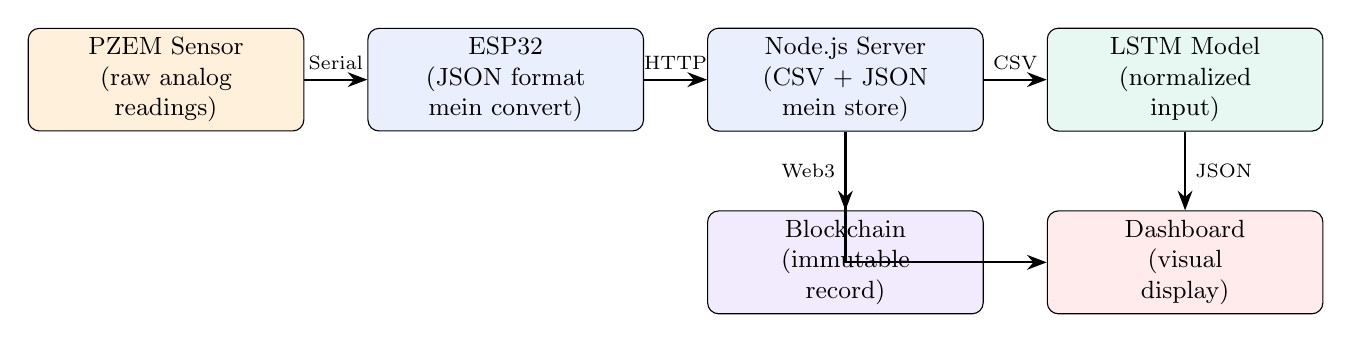
\begin{tikzpicture}[
    box/.style={draw, rounded corners, minimum width=3.5cm, minimum height=1.2cm, align=center, font=\small},
    arrow/.style={-{Stealth[length=2.5mm]}, thick}
]
\node[box, fill=warncolor!15] (pzem) {PZEM Sensor\\(raw analog\\readings)};
\node[box, fill=primaryblue!10, right=0.8cm of pzem] (esp) {ESP32\\(JSON format\\mein convert)};
\node[box, fill=primaryblue!10, right=0.8cm of esp] (srv) {Node.js Server\\(CSV + JSON\\mein store)};
\node[box, fill=accent!10, right=0.8cm of srv] (ml) {LSTM Model\\(normalized\\input)};

\draw[arrow] (pzem) -- node[above, font=\scriptsize] {Serial} (esp);
\draw[arrow] (esp) -- node[above, font=\scriptsize] {HTTP} (srv);
\draw[arrow] (srv) -- node[above, font=\scriptsize] {CSV} (ml);

\node[box, fill=codepurple!10, below=1cm of srv] (bc) {Blockchain\\(immutable\\record)};
\node[box, fill=red!8, below=1cm of ml] (dash) {Dashboard\\(visual\\display)};

\draw[arrow] (srv) -- node[left, font=\scriptsize] {Web3} (bc);
\draw[arrow] (ml) -- node[right, font=\scriptsize] {JSON} (dash);
\draw[arrow] (srv) |- (dash);

\end{tikzpicture}
\caption{Data Transformation Chain}
\end{figure}

Har step pe data ka format badalta hai:
\begin{itemize}[nosep]
    \item \textbf{PZEM $\rightarrow$ ESP32:} Analog electrical signals $\rightarrow$ digital numbers (Serial protocol)
    \item \textbf{ESP32 $\rightarrow$ Server:} Numbers $\rightarrow$ JSON format mein pack karke HTTP se bhejta hai
    \item \textbf{Server $\rightarrow$ CSV:} JSON $\rightarrow$ comma-separated values (AI training ke liye)
    \item \textbf{Server $\rightarrow$ Blockchain:} JSON $\rightarrow$ Solidity function call (Web3.js ke zariye)
    \item \textbf{AI $\rightarrow$ Dashboard:} Normalized prediction $\rightarrow$ real Watts mein convert $\rightarrow$ JSON response
\end{itemize}

\section{Technologies Summary}

\begin{table}[H]
\centering
\begin{tabularx}{\textwidth}{l l X}
\toprule
\textbf{Layer} & \textbf{Technology} & \textbf{Kyun Choose Kiya} \\
\midrule
Microcontroller & ESP32 & WiFi built-in hai, Arduino compatible, sasta hai \\
Power Sensor & PZEM-004T v3.0 & AC power accurately measure karta hai, serial interface easy hai \\
LCD & 1602A + I2C & Simple, sasta, I2C se sirf 2 wires chahiyen \\
Backend & Node.js + Express & JavaScript based, async operations mein fast, npm ecosystem \\
Blockchain & Solidity + Ganache & Ethereum standard, free local testing, strong tooling \\
Web3 & Web3.js v4.3 & Official Ethereum JS library \\
AI Model & TensorFlow/Keras & Industry standard, LSTM support, easy API \\
AI Server & Flask & Lightweight Python web server, ML ke saath integrate easy \\
Dashboard & Vanilla HTML/CSS/JS & No build step, instant deploy, zero dependencies \\
Tunneling & Ngrok & Free, instant public URL, HTTPS support \\
\bottomrule
\end{tabularx}
\caption{Technology Stack Aur Reasons}
\end{table}

\section{Code Size Summary}

\begin{table}[H]
\centering
\begin{tabular}{l r r l}
\toprule
\textbf{File} & \textbf{Lines} & \textbf{Size} & \textbf{Language} \\
\midrule
House A Firmware & 636 & 21.8 KB & C++ (Arduino) \\
House B Firmware & 393 & 11.5 KB & C++ (Arduino) \\
Backend Server & 811 & 24.7 KB & JavaScript \\
Dashboard & 1,095 & 46.6 KB & HTML/CSS/JS \\
Smart Contract & 278 & 8.9 KB & Solidity \\
Deploy Script & 134 & 4.9 KB & JavaScript \\
ML Trainer & 429 & 14.6 KB & Python \\
Prediction Server & 439 & 13.2 KB & Python \\
\midrule
\textbf{Total} & \textbf{$\sim$6,000} & \textbf{$\sim$160 KB} & \textbf{5 languages} \\
\bottomrule
\end{tabular}
\caption{Complete Codebase Size}
\end{table}

% ══════════════════════════════════════════════════
\chapter{System Startup \& Troubleshooting}
% ══════════════════════════════════════════════════

\section{Pehli Dafa Setup (First Time)}

Pehli baar system chalane se pehle kuch cheezein install aur configure karni padti hain:

\begin{enumerate}
    \item \textbf{Ganache Install Karo:} Ganache GUI download karo (trufflesuite.com/ganache), open karo, ``Quickstart Ethereum'' click karo. Yeh port 7545 pe local blockchain chalayega aur 10 fake Ethereum accounts dega.
    
    \item \textbf{Blockchain Deploy Karo:} \texttt{blockchain} folder mein jao, \texttt{npm install} karo (dependencies install hongi), phir deployment script chalao. Yeh contract Ganache pe deploy kare ga aur backend folder mein automatically sab configure kare ga.
    
    \item \textbf{Backend Setup:} \texttt{backend} folder mein \texttt{npm install} karo --- Express, Web3.js aur baqi dependencies install ho jayengi.
    
    \item \textbf{ML Setup:} \texttt{ml-model} folder mein Python packages install karo (\texttt{pip install -r requirements.txt}). Phir ya toh synthetic data generate karo ya real data se model train karo.
    
    \item \textbf{Firmware Flash:} \texttt{secrets.h.template} ko copy karke \texttt{secrets.h} banao, apne WiFi credentials aur server IP fill karo, Arduino IDE se dono ESP32 boards pe upload karo.
\end{enumerate}

\section{Rozana Startup Sequence (Daily)}

Har baar system chalane ke liye yeh \textbf{order follow karo} --- order important hai kyunke har cheez pichli cheez pe depend karti hai:

\begin{table}[H]
\centering
\begin{tabularx}{\textwidth}{c l X}
\toprule
\textbf{Step} & \textbf{Kya Karo} & \textbf{Kyun Pehle} \\
\midrule
1 & Ganache start karo & Blockchain chahiye sabse pehle kyunke backend isse connect hota hai \\
2 & Contract deploy karo & Agar Ganache restart kiya toh purana contract mit gaya --- naya chahiye \\
3 & Backend start karo & ESP32 data yahan bhejte hain --- pehle chalna chahiye ESP32 se \\
4 & AI server start karo & Optional --- backend iske bina bhi chalta hai \\
5 & Ngrok start karo & Sirf agar ESP32 remote hai (alag network pe) \\
6 & ESP32 boards power do & Sab servers pehle ready hone chahiyen \\
7 & Browser mein dashboard kholo & Sab chal raha ho toh \texttt{http://localhost:3000} pe dekho \\
\bottomrule
\end{tabularx}
\caption{Daily Startup Sequence --- Order Matters!}
\end{table}

\begin{warnbox}[Ganache Reset = Re-deploy!]
\textbf{Bahut important:} Har baar Ganache close karke dubara kholne pe purani chain \textbf{mit jati hai}. Toh contract dubara deploy karna padega. Backend bhi restart karo taake naya contract address load ho. Real blockchain mein yeh problem nahi hoti --- sirf development mein hai.
\end{warnbox}

\section{Dashboard Pe Kya Dikhna Chahiye}

Jab sab sahi chal raha ho toh dashboard ke navbar mein \textbf{3 green badges} dikhne chahiyen:

\begin{table}[H]
\centering
\begin{tabularx}{\textwidth}{l l X}
\toprule
\textbf{Badge} & \textbf{Green Kab} & \textbf{Red Kab} \\
\midrule
\textbf{Blockchain} & Ganache chal raha hai + contract deployed hai & Ganache band hai ya contract deploy nahi hua \\
\textbf{AI Engine} & Flask predict\_server.py chal raha hai & AI server band hai (predictions nahi aayengi) \\
\textbf{Live Feed} & ESP32 boards data bhej rahe hain & ESP32 powered off hai ya WiFi disconnect \\
\bottomrule
\end{tabularx}
\caption{Dashboard Status Badges}
\end{table}

\section{Config Files Reference}

\begin{table}[H]
\centering
\begin{tabularx}{\textwidth}{l X}
\toprule
\textbf{File} & \textbf{Kya Hai Aur Kab Change Karni Hai} \\
\midrule
\texttt{secrets.h} & WiFi password aur server IP. \textbf{Kab change:} WiFi change ho, PC ka IP change ho, ya Ngrok URL naya ho. \\
\texttt{.env} & Ganache URL aur contract address. \textbf{Kab change:} Deploy script automatically update karta hai. Manually tab change karo jab port ya network change ho. \\
\texttt{hardhat.config.js} & Blockchain network settings. \textbf{Kab change:} Normally kabhi nahi --- jab tak different network pe deploy na karna ho. \\
\texttt{requirements.txt} & Python packages list. \textbf{Kab change:} Naya Python package add karna ho toh. \\
\bottomrule
\end{tabularx}
\caption{Config Files --- Kab Kya Change Karna Hai}
\end{table}

\section{Common Problems Aur Solutions}

\begin{table}[H]
\centering
\begin{tabularx}{\textwidth}{X X}
\toprule
\textbf{Problem} & \textbf{Solution} \\
\midrule
Blockchain badge red hai & Ganache chal raha hai? Contract deploy kiya? Backend restart karo. \\
AI badge red hai & \texttt{python predict\_server.py} chalao. Model trained hai? Pehle \texttt{train\_model.py} chalao. \\
Live Feed red hai & ESP32 powered on hai? WiFi connected hai? Server ka IP sahi hai secrets.h mein? \\
PZEM NaN readings aa rahi hain & Wiring check karo --- TX aur RX swap toh nahi hain? PZEM ko power supply mil rahi hai? \\
LCD blank ya garbled hai & I2C address check karo (0x27 ya 0x3F?). SDA/SCL wires sahi pin pe hain? \\
Ngrok timeout error & Ngrok free plan mein URL har 2 ghante change hota hai. Naya URL generate karo aur secrets.h mein update karke re-flash karo. \\
Dashboard pe values 0.0 dikh rahe hain & Matlab ESP32 se data nahi aa raha. WiFi check karo, server URL check karo. \\
Model not loaded error & Pehle \texttt{python train\_model.py} chalao --- model train hona chahiye use karne se pehle. \\
Transaction blockchain pe record nahi ho rahi & Ganache mein ETH balance check karo. Contract address sahi hai .env mein? \\
\bottomrule
\end{tabularx}
\caption{Troubleshooting Guide}
\end{table}

\begin{tipbox}[Debugging Tip]
Agar kuch kaam nahi kar raha toh \textbf{terminal/console check karo}. Backend server terminal mein sab logs dikhata hai --- kya data aaya, kya blockchain pe gaya, kya error aayi. ESP32 ka Serial Monitor bhi sab status print karta hai. Logs padhna sabse fast debugging method hai.
\end{tipbox}


\end{document}
